\begin{thema}{Β}
Δίνεται η συνάρτηση $f(x) = a x^3 - \beta x^2 + 1$.
\begin{erwthma}
\item Το όριο $\lim_{x\to+\infty} \frac{f(x)}{x^3}$ ισούται με:
\[ \lim_{x\to+\infty} \frac{a x^3 - \beta x^2 + 1}{x^3} = \lim_{x\to+\infty} \frac{a x^3}{x^3} = a \]
Αφού το όριο δίνεται ίσο με 2, προκύπτει $a=2$.
Η συνάρτηση είναι $f(x) = 2x^3 - \beta x^2 + 1$. Είναι πολυωνυμική, άρα παραγωγίσιμη με $f'(x) = 6x^2 - 2\beta x$.
Γνωρίζουμε ότι η $f$ παρουσιάζει τοπικό ακρότατο στο $x_0 = 1$. Σύμφωνα με το θεώρημα Fermat, πρέπει να ισχύει $f'(1) = 0$.
\[ f'(1) = 0 \Leftrightarrow 6(1)^2 - 2\beta(1) = 0 \Leftrightarrow 6 - 2\beta = 0 \Leftrightarrow 2\beta = 6 \Leftrightarrow \beta = 3 \]
Άρα $a=2$ και $\beta=3$, και ο τύπος είναι $f(x) = 2x^3 - 3x^2 + 1$.

\item Υπολογίζουμε τη δεύτερη παράγωγο:
\[ f''(x) = (6x^2 - 6x)' = 12x - 6 \]
Μηδενίζουμε τη δεύτερη παράγωγο για να βρούμε τα σημεία καμπής:
\[ f''(x) = 0 \Leftrightarrow 12x = 6 \Leftrightarrow x = \frac{1}{2} \]
Στον παρακάτω πίνακα φαίνεται το πρόσημο της $f''$ και η κυρτότητα:
\begin{center}
\begin{tikzpicture}
\tkzTabInit[color,lgt=2,espcl=1.5,colorC = red7,colorL = red9,colorV = red7]%
{$x$ / .8,$f''(x)$ /0.8,$f(x)$/0.8}%
{$-\infty$,$1/2$,$+\infty$}%
\tkzTabLine{ , -, z, +, }
\tkzTabLine{ , \curvearrowright, t, \rotatebox[origin= c]{180}{$\curvearrowleft$}, }
\end{tikzpicture}
\end{center}
Άρα η $f$ είναι κοίλη (στρέφει τα κοίλα κάτω) στο $(-\infty, \frac{1}{2}]$, και κυρτή (στρέφει τα κοίλα άνω) στο $[\frac{1}{2}, +\infty)$. Το $x=1/2$ είναι σημείο καμπής.

\item Θεωρούμε τη συνάρτηση $f$ στο κλειστό $[-1, 0]$, στην οποία είναι συνεχής. Στα άκρα έχουμε:
- $f(-1) = 2(-1)^3 - 3(-1)^2 + 1 = -2 - 3 + 1 = -4 < 0$.
- $f(0) = 2(0)^3 - 3(0)^2 + 1 = 1 > 0$.
Από το Θεώρημα Bolzano εξασφαλίζεται ότι υπάρχει τουλάχιστον ένα $x_0 \in (-1, 0)$ τέτοιο ώστε $f(x_0)=0$.

\item Αναζητούμε σημείο επαφής $(x_1, f(x_1))$ στο οποίο η εφαπτομένη να είναι παράλληλη προς την $\varepsilon: y = 12x-5$. 
Ο συντελεστής διεύθυνσης της $\varepsilon$ είναι $\lambda = 12$. Συνεπώς πρέπει $f'(x_1) = 12$.
\[ 6x_1^2 - 6x_1 = 12 \Leftrightarrow x_1^2 - x_1 - 2 = 0 \]
Με παράγοντες έχουμε $(x_1 - 2)(x_1 + 1) = 0$, άρα οι ρίζες είναι $x_1 = 2$ και $x_1 = -1$.
Για $x_1 = 2$: Το σημείο επαφής είναι $(2, f(2))$ με $f(2) = 16 - 12 + 1 = 5$.
Η εξίσωση της εφαπτομένης είναι $y - f(2) = f'(2)(x-2) \Leftrightarrow y - 5 = 12(x-2) \Leftrightarrow y = 12x - 24 + 5 \Leftrightarrow y = 12x - 19$.
Για $x_1 = -1$: Το σημείο επαφής είναι $(-1, f(-1))$ με $f(-1) = -4$ (από το προηγούμενο ερώτημα).
Η εξίσωση της εφαπτομένης είναι $y - f(-1) = f'(-1)(x+1) \Leftrightarrow y + 4 = 12(x+1) \Leftrightarrow y = 12x + 12 - 4 \Leftrightarrow y = 12x + 8$.
Άρα υπάρχουν δύο τέτοιες εφαπτόμενες.
\end{erwthma}
\end{thema}
